\documentclass[10pt,twocolumn,letterpaper]{article}

\usepackage{cvpr}
\usepackage{times}
\usepackage{epsfig}
\usepackage{graphicx}
\usepackage{amsmath}
\usepackage{amssymb}
\usepackage{enumitem}


\usepackage{listings}
\usepackage{color}

\definecolor{dkgreen}{rgb}{0,0.6,0}
\definecolor{gray}{rgb}{0.5,0.5,0.5}
\definecolor{mauve}{rgb}{0.58,0,0.82}

\lstset{frame=tb,
  language=Python,
  aboveskip=3mm,
  belowskip=3mm,
  showstringspaces=false,
  columns=flexible,
  basicstyle={\small\ttfamily},
  numbers=none,
  numberstyle=\tiny\color{gray},
  keywordstyle=\color{blue},
  commentstyle=\color{dkgreen},
  stringstyle=\color{mauve},
  breaklines=true,
  breakatwhitespace=true,
  tabsize=3
}

% Include other packages here, before hyperref.

% If you comment hyperref and then uncomment it, you should delete
% egpaper.aux before re-running latex.  (Or just hit 'q' on the first latex
% run, let it finish, and you should be clear).
\usepackage[breaklinks=true,bookmarks=false]{hyperref}

\cvprfinalcopy % *** Uncomment this line for the final submission

\def\cvprPaperID{****} % *** Enter the CVPR Paper ID here
\def\httilde{\mbox{\tt\raisebox{-.5ex}{\symbol{126}}}}

% Pages are numbered in submission mode, and unnumbered in camera-ready
%\ifcvprfinal\pagestyle{empty}\fi
\setcounter{page}{1}
\begin{document}

%%%%%%%%% TITLE
\title{Traffic Anomalies Detection Based on Objective's State Estimation}
\author{
Daniel Shumaker\\
Michigan State University\\
{\tt\small shumak37@msu.edu}
% For a paper whose authors are all at the same institution,
% omit the following lines up until the closing ``}''.
% Additional authors and addresses can be added with ``\and'',
% just like the second author.
% To save space, use either the email address or home page, not both
\and
Luan Nguyen\\
Michigan State University\\
{\tt\small nguye590@msu.edu}
\and
Pengyu Chu\\
Michigan State University\\
{\tt\small chupengy@msu.edu}
}

\maketitle
%\thispagestyle{empty}

%%%%%%%%% ABSTRACT
%\begin{abstract}
%   The ABSTRACT is to be in fully-justified italicized text, at the top
%   of the left-hand column, below the author and affiliation
%   information. Use the word ``Abstract'' as the title, in 12-point
%   Times, boldface type, centered relative to the column, initially
%   capitalized. The abstract is to be in 10-point, single-spaced type.
%   Leave two blank lines after the Abstract, then begin the main text.
%   Look at previous CVPR abstracts to get a feel for style and length.
%\end{abstract}

\section{Problem Description}
    
Our project comes from \textit{aicitychallenge.org}: a competition held every year that challenges programmers to expand our society's knowledge in the realm of self driving cars with a focus on urban car automation. Every year they offer new challenges; our project is based on challenge number 3. The challenge we are tackling is called "Traffic Anomaly Detection". Like the name suggests, our challenge is to detect behavior that deviates from the way vehicles normally act. Examples of anomalies we will be looking for are illegal lane crossing, wrong direction driving, swerving cars, illegal U-turns, stopped vehicles, and crashes with a few stretch goals like detecting the lack of headlight usage and excessive breaking. Our ability to detect those will depend heavily on the data set quality. While we may want to create a program that detects all these things, it will be hard to know for sure if the data never includes them. While this is called a city challenge, most of the videos we've seen in the data set are set on a highway; a place where U-turns detection will be hard to train due to the infrequency of their occurrence in that setting.

This problem is important because it can help save the lives of people as cars more and more become autonomous. With sensors tracking traffic, signaling systems, and infrastructure, our transportation systems are becoming smarter. With computer vision and deep learning, there are many opportunities to solve real-world problems with data gained from multi-cameras. The major causes of accidents are the outliers to normal drivers. The drivers that go much slower on the free way, that aggressively change lanes, and ride others' bumpers are a major cause for sober accidents. Another major accident is caused by drivers under the influence of drugs. These drivers have a differing, and more dangerous set of driving patterns. Both groups can be extremely dangerous, particularly in traffic highways and intersections. With software that can detect anomalies in behavior, a computer could spot potential hazards and, depending on where it is implemented, could notify police in the area of a potentially drunk driver, or could tell an autonomous vehicle which cars to give a wide berth to. Solutions could potentially get the humans in the loop to pay attention to meaningful visual information in situations where timely intervention can save lives.\cite{naphade2017nvidia}

Unfortunately, progress has so far been limited for several reasons like missing data labels, and the lack of high-quality models that convert data to decent forms. In other words, it is hard to get data with labels from the real world. Due to the lack of labels, anomalies cannot be classified with current algorithms. Thus, we plan to seek a public dataset with annotations to address this problem and focus on the research and development of techniques that rely more on the state-of-the-art object detection and transfer learning.

With some pre-trained model like VGG 16 \cite{ren2015faster}, we can leverage transfer learning to combine these models with our approach and detect the abnormal traffic behaviors from traffic camera video data which is provided by NVIDIA corporation.

\section{Dataset}

Our solution to the problem described above begins with the data set we have to work with. \textit{AI City Challenge} provided us with the data for this challenge. They provided both a training and test set for us to use, and both sets are visually pretty similar. Each folder contains 100 mp4 files in them. Each video is about 15 minutes long, usually is set in a highway, and, not surprisingly, has a lot of cars in it. In the README file for the training videos, the challengers give us the areas they believe to have issues. Surprisingly, most videos in these sets don't have any anomalies in them, or at least were not recorded in the README document. 

After looking at a few videos, we made a few observations about the quality of the data. It is very likely that there will be wind, and the video will need to be stabilized before processing. The cameras used to record the videos differ in quality greatly. Weather conditions vary, the time of day the filming took place varies, geographical location varies, and the angle the cameras filmed from varies too. Even though this is called the "city challenge", much of these videos take place on highways. Another observation we made after looking at the videos and at the suggested anomalies of the training videos was a lack of diversity in the errors. Much of the errors that occur are vehicles stopped on the sides of the road, and many of the errors that weren't about stalled vehicles, didn't appear to have any errors at all.

Apart from those observations, our data looks great! We will just need to be wary, and preprocess the data a good amount. Here are a few images from the videos given to us in the data set seed in Figure [\ref{train17}] [\ref{train41}]. Here is an example of an image with anomalies in Figure [\ref{train2}] and [\ref{train11}]

\begin{figure}  
    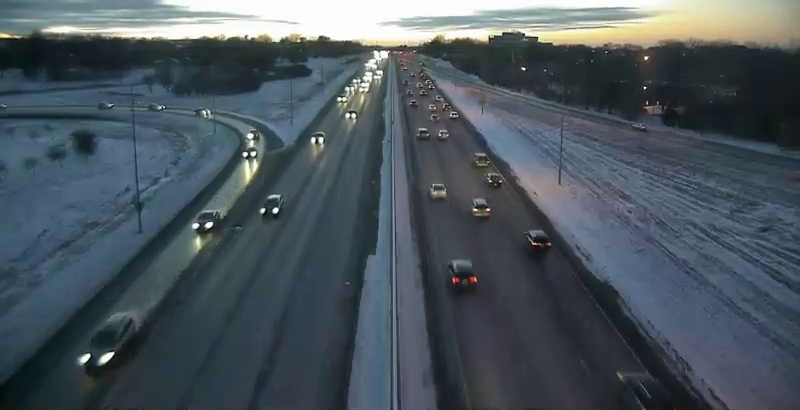
\includegraphics[scale=.29]{images/anomalyTrain17.png}
    \caption{Image from video 17}
    \label{train17}
\end{figure}

\begin{figure}  
    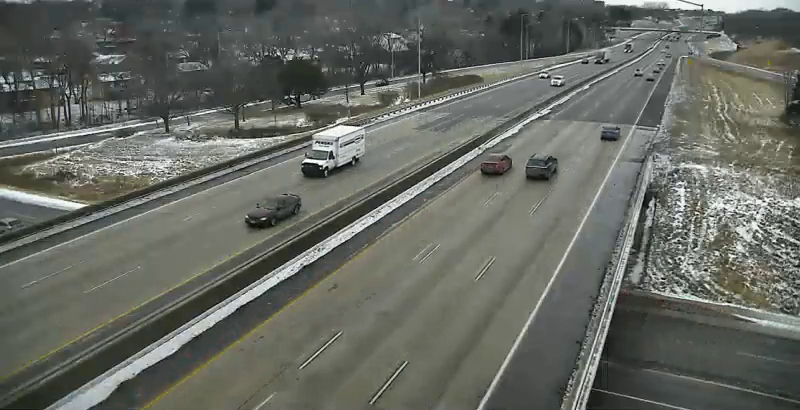
\includegraphics[scale=.29]{images/anomalyTrain41.png}
    \caption{Image from video 41}
    \label{train41}
\end{figure}

\begin{figure}  
    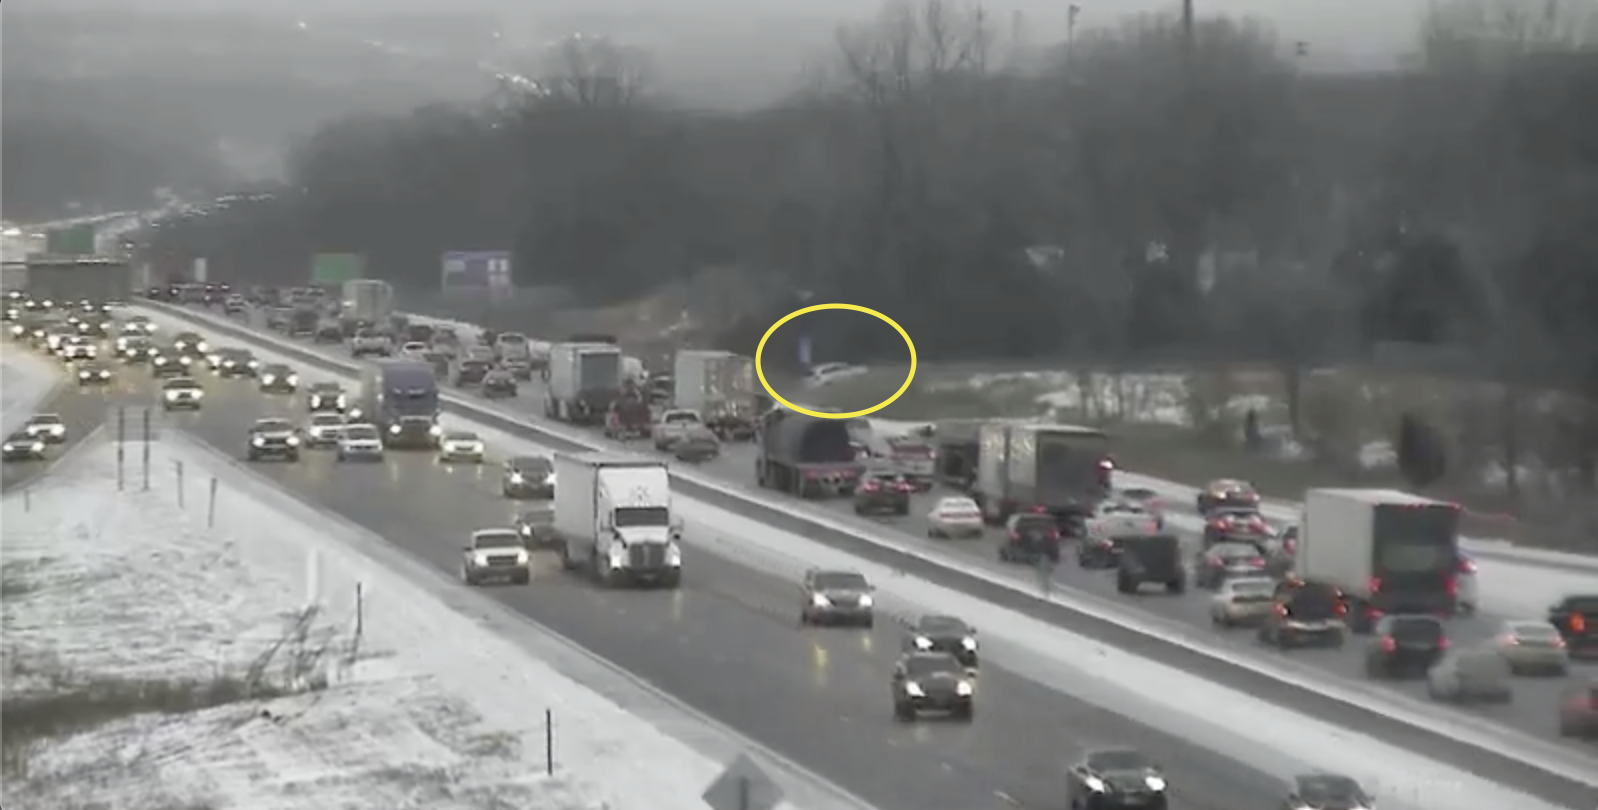
\includegraphics[width=8.2cm]{images/anomalyTrain11.png}
    \caption{Image from video 11. Contains Anomalies. In the yellow circle, the car ran off the road}
    \label{train11}
\end{figure}

\begin{figure}  
    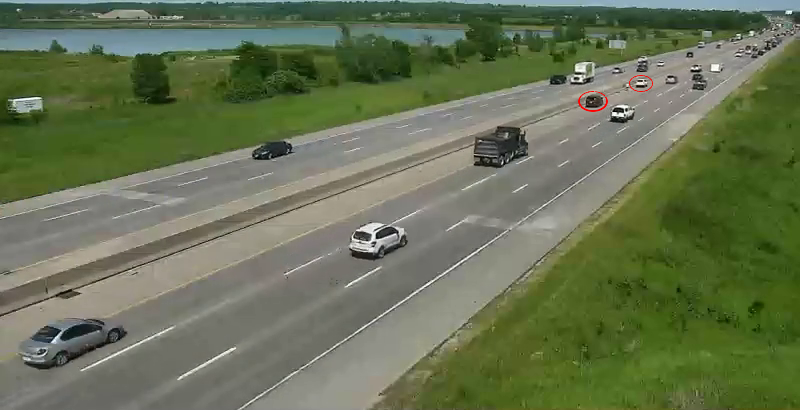
\includegraphics[scale=.29]{images/anomalyTrain2_focus.png}
    \caption{Image from video 2. Contains Anomalies. In the small red circles, two cars are stopped on the side of the road.}
    \label{train2}
\end{figure}


The challengers require that we report our anomalies in the same way that they do: give the video name, the start time of the anomaly, and the end time of it in seconds. If the anomaly continues past the end of the video, we are to give the last second of the video as the stopping time.


\section{Methodology}

Based on the definition of anomalies, we mainly have two types of anomalies, which are running off the road and stalling on the highway road. After reviewing some literatures, we find an effective workflow can address this problem:
1) We should detect every cars or trucks in the videos and point out their locations; 2) Track these vehicles in the sequence of each video; 3) Measure the speed of cars based on a continues frames in the videos and judge its status; 4) Detect the road area to check whether a car runs off the road or not.


In this section, I'll introduce our methods mentioned in details.

\subsection{Vehicle Detection}

In the realm of objective detection, we have lots of state-of-the-art methods including two-stage detection methods like Faster R-CNN \cite{ren2015faster} or one-stage detection represented by YOLOv3\cite{redmon2018yolov3}
and SSD\cite{liu2016ssd}. After a comparison among these methods, we choose the Mask R-CNN as our detector because it has the best accuracy over the benchmark.\cite{DBLP:journals/corr/HeGDG17}.
	
\subsubsection{Pre-trained Mask R-CNN and Applied in Videos}

It's hard to train a CNN model from scratch, so we leverage the pre-trained model in COCO dataset\cite{DBLP:journals/corr/LinMBHPRDZ14}, which is a public images dataset, to detect cars in our scene. On the other hand, Mask R-CNN is a classifier based on the image nor video, so we need to modify it to be deployed on the videos. 
	
	We use a video library named 'moviepy' to deal with these videos and after extracting a sequence of frames from the video, we apply the detector on each frame. The details will be displayed in the codes. The Figure \ref{seq_cars} displays a continuous result. 
	
	\begin{figure}  
    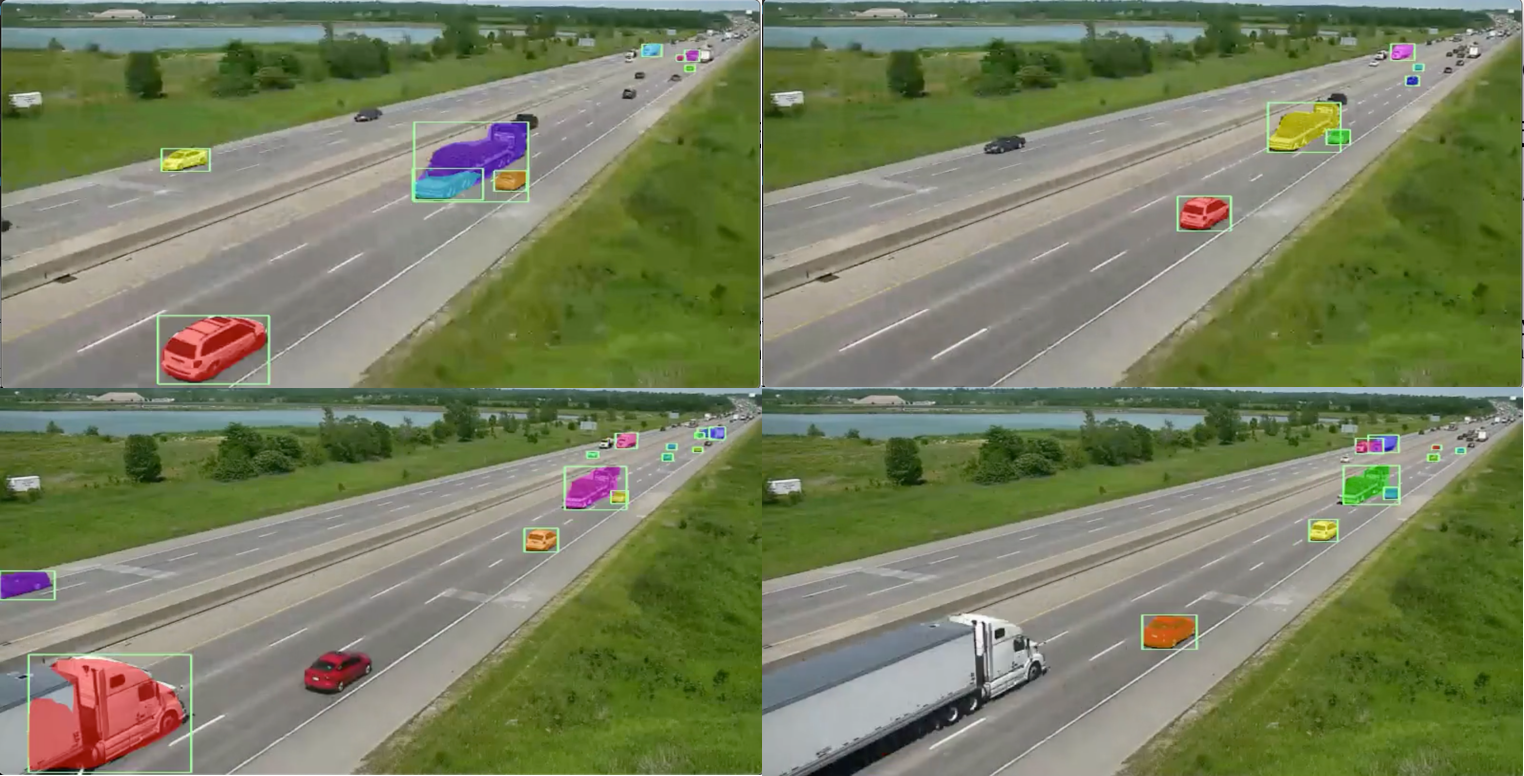
\includegraphics[width=8cm]{images/car.png}
    \caption{Detect cars through videos with Mask R-CNN. The sequence is from left to right and top to down.}
    \label{seq_cars}
	\end{figure}

	
	Finally, we output our detections as a text file for each video, consisting of labels and bounding boxes coordinates. The format is exhibited in the following table. 
	
	\begin{lstlisting}
1,-1,320,24,640,431,-1,-1,-1
1,-1,234,868,257,887,-1,-1,-1
1,-1,158,30,951,969,-1,-1,-1
1,-1,153,833,217,875,-1,-1,-1
1,-1,301,476,341,520,-1,-1,-1
1,-1,248,768,282,793,-1,-1,-1
2,-1,320,24,640,431,-1,-1,-1
2,-1,234,868,257,887,-1,-1,-1
	\end{lstlisting}
	
\subsection{Vehicle Tracking}

During the vehicle tracking, we leverage a relative mature method, Simple Online and Realtime Tracking (SORT)\cite{bewley2016simple} after consider the realtime performance we need. The basis of the algorithm is that it compares a frame with the next one among the coordinates and size of bounding boxes , and then compute a velocity vector. More specifically, they use the following flows to process the calculation:

1) It uses Kalman filters to compute the velocity factor. Kalman filter is essentially doing some math to smooth the velocity and direction computation by comparing the predicted state and the real detection given by Faster R-CNN. Obviously, we changes it to a better model Mask R-CNN;

2) Its uses an assignment cost matrix that is computed as the intersection over union (IOU) distance between each detection and all predicted bounding boxes from the existing targets (which is putting all the dimensions in a normalized matrix). Then the best match is computed using the Hungarian Algorithm, which is a way to fast compute lots of matrices;

3) It also deals with the score of the detections which other tracking methods don't use. Then the tracker could choose between two close detections based on that.

After we use SORT to track our targets, we get an example like the following table:

	\begin{lstlisting}
1,1887,1252.28,509.20,59.49,133.61,1,-1,-1,-1
1,1886,1869.09,376.41,49.91,222.56,1,-1,-1,-1
1,1885,19.57,469.71,87.46,343.43,1,-1,-1,-1
...
2,1886,1875.44,376.36,43.85,201.27,1,-1,-1,-1
2,1885,11.99,481.75,104.02,385.41,1,-1,-1,-1
...
3,1887,1248.68,487.23,56.65,162.73,1,-1,-1,-1
3,1886,1875.18,376.38,43.39,197.06,1,-1,-1,-1
3,1885,-7.56,337.99,127.29,553.51,1,-1,-1,-1
...
4,1886,1873.05,374.18,45.00,200.53,1,-1,-1,-1
4,1885,-9.25,295.41,126.77,598.18,1,-1,-1,-1
...
5,1886,1870.62,364.84,47.16,205.23,1,-1,-1,-1
5,1885,-8.11,257.61,129.29,646.33,1,-1,-1,-1
	\end{lstlisting}
	
Compared to the last section output, the tracker annotates the identity for each car. Based on the example, we can see id=1885 and id=1886 are moving in this five frames and the id=1887 disappears after the third frame. We can exploit the moving information to valid the car stalls or not and whether it's included in the road area or not.


\subsection{Speed Validation}

After vehicle tracking, we can a sequence of each car that we've tracked in the last section. Assume the sequence is true (since we still face some tracking errors but we'll address it with a direction limitation in the next work.). Since the camera position and perspective won't change, we can use the motion of the target centroid and the gap between frames in the videos to calculate the speed.

$$P(x, y) = \frac{(Box_{11} +  Box_{12} + Box_{11} +  Box_{22})}{4}$$

$$D(t) = \Sigma_{i=0}^{k}\frac{P_{t-i}}{k+1}$$

$$V(t) = \frac{D(t)}{gap}$$

\[
    h(x)= 
\begin{cases}
    1,& \text{if } V(t) > threshold\\
    0,              & \text{otherwise}
\end{cases}
\]
$P(x,y)$ is the representation of a target centroid, $D(t)$ is the average moving distance, and $V(t)$ represent the speed of pixels motion with the gap depending on the extracting rate from videos. The $h(x)$ classifies the anomalies and threshold is up to the training results. So from this equation $h(x)$, we can know a car stalls or not in the time $t$


\subsection{Road Detection}

Our cameras are all fixed and then that means the road will be static as the background. So we can use a simple algorithm Canny Edge Detection and Hough Transform to estimate the road areas in the each video. That's our subsequent work to finish.

After that, we'll compare whether the centroid of a car is in the area or not and then valid it ran off the road or not, which is the other type of anomalies. 

$$P(x, y) = \frac{(Box_{11} +  Box_{12} + Box_{11} +  Box_{22})}{4}$$
\[
    f(x)= 
\begin{cases}
    1,& \text{if } x\in Region_{road}\\
    0,              & \text{otherwise}
\end{cases}
\]

In this equation, P(x,y) represents the coordinates of the centroid of each car and $Region_{road}$ can be depicted with 0-1 Matrix. So the $f(P(x, y))$ will express whether it's an anomaly or not.

\section{Next Work}

Since there are not annotations in our dataset, so we have to do annotations work by ourselves to improve the performance of our Machine Learning models. That's the most importance part because our tracker is totally depending on the the results of detectors. Then we need implement the road detection algorithm even though we have the specific theorem. After completing the above work, we need to apply our algorithm on the testing dataset and evaluate it through F1 Score Method \cite{aicitychallenge}. The remaining work is listed:

\begin{itemize}[topsep=0pt, itemsep=-5pt]
   \item Train the CNN model based on our own dataset;
   \item implement the static road detection and form a road matrix for each video;
   \item Apply the algorithm on the testing dataset;
   \item Evaluate the results with a formal standard.
\end{itemize}



{\small
\bibliographystyle{ieee}
\bibliography{egbib}
}

\end{document}
